
\definecolor{cb3b3b3}{RGB}{179,179,179}
\definecolor{cff8080}{RGB}{255,128,128}
\definecolor{c2c5aa0}{RGB}{44,90,160}


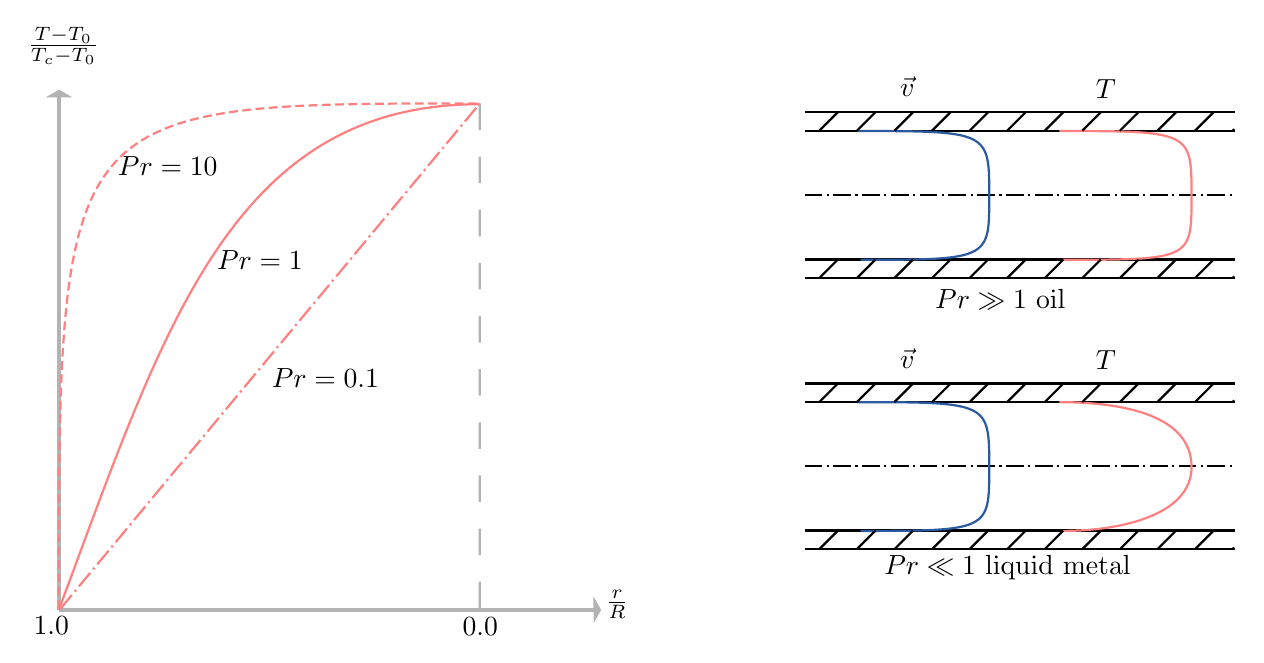
\begin{tikzpicture}[y=0.80pt, x=0.8pt,yscale=-1, inner sep=0pt, outer sep=0pt]
\begin{scope}[shift={(0,-782.35975)}]
  \begin{scope}[shift={(0,774.35975)},fill=black]
  \end{scope}
  \path[fill=cb3b3b3] (254.6422,1030.9418) -- (258.1554,1037.0269) --
    (254.7091,1042.9960) -- cycle;
  \path[draw=cb3b3b3,line join=miter,line cap=butt,miter limit=4.00,line
    width=1.600pt] (13.2229,803.7281) -- (13.2229,1036.9689)(255.6121,1036.9689)
    -- (13.2229,1036.9689);
  \path[fill=cb3b3b3] (7.1958,805.5497) -- (13.2809,802.0365) --
    (19.2500,805.4828) -- cycle;
  \path[color=black,fill=cb3b3b3,line width=0.800pt] (202.8125,820.2697) --
    (203.8125,820.2697) -- (203.8125,808.2697) -- (202.8125,808.2697) --
    cycle(202.8125,844.2697) -- (203.8125,844.2697) -- (203.8125,832.2697) --
    (202.8125,832.2697) -- cycle(202.8125,868.2697) -- (203.8125,868.2697) --
    (203.8125,856.2697) -- (202.8125,856.2697) -- cycle(202.8125,892.2697) --
    (203.8125,892.2697) -- (203.8125,880.2697) -- (202.8125,880.2697) --
    cycle(202.8125,916.2697) -- (203.8125,916.2697) -- (203.8125,904.2697) --
    (202.8125,904.2697) -- cycle(202.8125,940.2697) -- (203.8125,940.2697) --
    (203.8125,928.2697) -- (202.8125,928.2697) -- cycle(202.8125,964.2697) --
    (203.8125,964.2697) -- (203.8125,952.2697) -- (202.8125,952.2697) --
    cycle(202.8125,988.2697) -- (203.8125,988.2697) -- (203.8125,976.2697) --
    (202.8125,976.2697) -- cycle(202.8125,1012.2698) -- (203.8125,1012.2698) --
    (203.8125,1000.2697) -- (202.8125,1000.2697) -- cycle(202.8125,1036.2696) --
    (203.8125,1036.2696) -- (203.8125,1024.2696) -- (202.8125,1024.2696) -- cycle;
  \path[fill=black] (195.51093,1048.4893) node[above right] (text3075-4-1-2-9)
    {$0.0$};
  \path[fill=black] (260.02991,1040.9917) node[above right] (text3075-4-1-2-9-9)
    {$\frac{r}{R}$};
  \path[fill=black] (-0.89976788,790.70367) node[above right]
    (text3075-4-1-2-9-9-7) {$\frac{T-T_{0}}{T_{c}-T_{0}}$};
  \path[fill=black] (1.7341394,1048.0874) node[above right] (text3075-4-1-2-9-91)
    {$1.0$};
  \path[shift={(0,782.35975)},draw=cff8080,line join=miter,line cap=butt,line
    width=0.800pt] (13.1755,254.6286) .. controls (60.3876,127.9977) and
    (91.1303,26.2538) .. (203.1219,26.2538);
  \path[shift={(0,782.35975)},draw=cff8080,dash pattern=on 3.20pt off 1.60pt,line
    join=miter,line cap=butt,miter limit=4.00,line width=0.800pt]
    (13.1755,254.2626) .. controls (13.1755,25.8814) and (13.0521,25.8878) ..
    (203.4878,25.8878);
  \path[shift={(0,782.35975)},draw=cff8080,dash pattern=on 6.40pt off 1.60pt on
    0.80pt off 1.60pt,line join=miter,line cap=butt,miter limit=4.00,line
    width=0.800pt] (13.9175,254.0943) -- (203.2953,25.9462);
  \path[shift={(0,782.35975)},fill=black] (109.35199,154.18631) node[above right]
    (text3832) {$Pr=0.1$};
  \path[fill=black] (84.627068,883.2522) node[above right] (text3832-6) {$Pr=1$};
  \path[fill=black] (39.892166,841.00262) node[above right] (text3832-4)
    {$Pr=10$};
  \path[draw=black,line join=miter,line cap=butt,line width=0.800pt]
    (350.0000,820.7324) -- (544.2747,820.7324)(350.0000,812.2825) --
    (544.2747,812.2825);
  \path[draw=black,line join=miter,line cap=butt,line width=0.800pt]
    (350.0000,887.1716) -- (544.2747,887.1716)(350.0000,878.7217) --
    (544.2747,878.7217);
  \path[draw=black,dash pattern=on 6.40pt off 1.60pt on 0.80pt off 1.60pt,line
    join=miter,line cap=butt,miter limit=4.00,line width=0.800pt]
    (350.0000,849.7270) -- (544.2747,849.7270);
  \path[draw=cff8080,line join=miter,line cap=butt,line width=0.800pt]
    (465.1487,820.7324) .. controls (524.7955,820.7324) and (524.7953,820.8811) ..
    (524.7953,850.0586) .. controls (524.7953,878.5954) and (525.0365,878.8877) ..
    (466.6399,878.8877);
  \path[draw=c2c5aa0,line join=miter,line cap=butt,line width=0.800pt]
    (373.7850,820.7324) .. controls (433.4317,820.7324) and (433.4315,820.8811) ..
    (433.4315,850.0586) .. controls (433.4315,878.5954) and (433.6727,878.8877) ..
    (375.2761,878.8877);
  \path[fill=black] (409.00256,901.31171) node[above right] (text3957) {$Pr \gg 1$
    oil};
  \path[shift={(0,782.35975)},fill=black] (393.1701,22.963923) node[above right]
    (text3961) {$\vec{v}$};
  \path[shift={(0,782.35975)},fill=black] (481.64578,23.460978) node[above right]
    (text3965) {$T$};
  \path[draw=black,line join=miter,line cap=butt,line width=0.800pt]
    (350.0000,943.1856) -- (544.2747,943.1856)(350.0000,934.7356) --
    (544.2747,934.7356);
  \path[draw=black,line join=miter,line cap=butt,line width=0.800pt]
    (350.0000,1009.6248) -- (544.2747,1009.6248)(350.0000,1001.1749) --
    (544.2747,1001.1749);
  \path[draw=black,dash pattern=on 6.40pt off 1.60pt on 0.80pt off 1.60pt,line
    join=miter,line cap=butt,miter limit=4.00,line width=0.800pt]
    (350.0000,972.1802) -- (544.2747,972.1802);
  \path[draw=cff8080,line join=miter,line cap=butt,line width=0.800pt]
    (465.1488,943.1856) .. controls (494.4752,943.1856) and (524.7953,949.2990) ..
    (524.7953,972.5118) .. controls (524.7953,993.5927) and (494.2191,1001.3409)
    .. (466.6399,1001.3409);
  \path[draw=c2c5aa0,line join=miter,line cap=butt,line width=0.800pt]
    (373.7850,943.1856) .. controls (433.4318,943.1856) and (433.4315,943.3343) ..
    (433.4315,972.5118) .. controls (433.4315,1001.0485) and (433.6727,1001.3409)
    .. (375.2761,1001.3409);
  \path[fill=black] (386.00354,1023.2678) node[above right] (text3957-2) {$Pr \ll
    1$ liquid metal};
  \path[fill=black] (393.17014,927.77686) node[above right] (text3961-1)
    {$\vec{v}$};
  \path[fill=black] (481.64581,928.27393) node[above right] (text3965-8) {$T$};
  \path[rounded corners=0.0000cm] (349.9927,812.1168) rectangle
    (544.0262,821.0969);
  \path[shift={(0,782.35975)},rounded corners=0.0000cm] (259.1145,8.0854)
    rectangle (320.9315,28.1167);
\end{scope}
  \path[rounded corners=0.0000cm] (350.2246,29.8398) rectangle (544.0759,38.2401);
  \path[draw=black,line width=0.800pt] (365.0599,29.8398) --
    (356.6596,38.2401)(373.6302,38.2401) -- (382.0304,29.8398)(399.0010,29.8398)
    -- (390.6008,38.2401)(407.5713,38.2401) --
    (415.9715,29.8398)(432.9421,29.8398) -- (424.5419,38.2401)(441.5125,38.2401)
    -- (449.9127,29.8398)(466.8832,29.8398) --
    (458.4830,38.2401)(475.4536,38.2401) -- (483.8538,29.8398)(500.8244,29.8398)
    -- (492.4241,38.2401)(509.3947,38.2401) --
    (517.7949,29.8398)(534.7655,29.8398) -- (526.3653,38.2401)(543.3358,38.2401)
    -- (544.0759,37.5000);
\begin{scope}[shift={(0,66.54695)}]
  \path[rounded corners=0.0000cm] (350.2246,29.8398) rectangle (544.0759,38.2401);
  \path[draw=black,line width=0.800pt] (365.0599,29.8398) --
    (356.6596,38.2401)(373.6302,38.2401) -- (382.0304,29.8398)(399.0010,29.8398)
    -- (390.6008,38.2401)(407.5713,38.2401) --
    (415.9715,29.8398)(432.9421,29.8398) -- (424.5419,38.2401)(441.5124,38.2401)
    -- (449.9127,29.8398)(466.8832,29.8398) --
    (458.4830,38.2401)(475.4536,38.2401) -- (483.8538,29.8398)(500.8244,29.8398)
    -- (492.4241,38.2401)(509.3947,38.2401) --
    (517.7949,29.8398)(534.7655,29.8398) -- (526.3653,38.2401)(543.3358,38.2401)
    -- (544.0759,37.5000);
\end{scope}
\begin{scope}[shift={(0,122.56091)}]
  \path[rounded corners=0.0000cm] (350.2246,29.8398) rectangle (544.0759,38.2401);
  \path[draw=black,line width=0.800pt] (365.0599,29.8398) --
    (356.6596,38.2401)(373.6302,38.2401) -- (382.0304,29.8398)(399.0010,29.8398)
    -- (390.6008,38.2401)(407.5713,38.2401) --
    (415.9715,29.8398)(432.9421,29.8398) -- (424.5419,38.2401)(441.5124,38.2401)
    -- (449.9127,29.8398)(466.8832,29.8398) --
    (458.4830,38.2401)(475.4536,38.2401) -- (483.8538,29.8398)(500.8244,29.8398)
    -- (492.4241,38.2401)(509.3947,38.2401) --
    (517.7949,29.8398)(534.7655,29.8398) -- (526.3653,38.2401)(543.3358,38.2401)
    -- (544.0759,37.5000);
\end{scope}
\begin{scope}[shift={(0,189.00015)}]
  \path[rounded corners=0.0000cm] (350.2246,29.8398) rectangle (544.0759,38.2401);
  \path[draw=black,line width=0.800pt] (365.0599,29.8398) --
    (356.6596,38.2401)(373.6302,38.2401) -- (382.0304,29.8398)(399.0010,29.8398)
    -- (390.6008,38.2401)(407.5713,38.2401) --
    (415.9715,29.8398)(432.9421,29.8398) -- (424.5419,38.2401)(441.5124,38.2401)
    -- (449.9127,29.8398)(466.8832,29.8398) --
    (458.4830,38.2401)(475.4536,38.2401) -- (483.8538,29.8398)(500.8244,29.8398)
    -- (492.4241,38.2401)(509.3947,38.2401) --
    (517.7949,29.8398)(534.7655,29.8398) -- (526.3653,38.2401)(543.3358,38.2401)
    -- (544.0759,37.5000);
\end{scope}

\end{tikzpicture}
